\kommentar{EMV}

\begin{karte}{Was bedeutet EMV?}
	EMV steht für Elektomagnetische Verträglichkeit. Das bedeutet im Wesentlichen, dass das Gerät in einem Umfeld mit gewissen Störungen störungsfrei funktioniert aber auch dass das Gerät das Umfeld nicht zu stark stört. Ein wenig Stören ist erlaubt. Dies ist von der Kategorie abhängig.
\end{karte}

\begin{karte}{Welche drei Perspektiven gibt es im Zusammenhang mit EMV?}
	Die drei Perspektiven sind \textbf{SI}, \textbf{PI} und \textbf{EMC}.\\[5pt]
	\textbf{SI} steht für Signal Integrity und behandlet vorallem die Frage, Wie gut sind die Signale intern. Werden alle Anforderungen bezüglich den standardisierten Signalen eingehalten?\\[5pt]
	\textbf{PI} steht für Power Integrity. Das ist die Koexistens Intern. Die Verschieden Teile eines System dürfen sich nicht zu viel stören. Ein bisschen Störung ist allerdings nicht zu vermeiden. Die Störungen werden primär durch die gesamte Leistungs-/Energieversorgung von einem Teil auf den Anderen übertragen.\\[5pt]
	\textbf{EMC} steht für Electromagnetic Compatibility. Das ist die Koexistenz gegen Aussen.
\end{karte}

\begin{karte}{Was beinhaltet das Grundmodell der Störungsbeeinflussung?}
	Das Grundmodell basiert auf drei Komponenten. Es gibt Störquellen, Kopplungspfade und Störsenken.\\
	%\scalebox{.7}{%Autor: Simon Walker
%Version: 1.0
%Datum: 29.06.2020
%Lizenz: CC BY-NC-SA


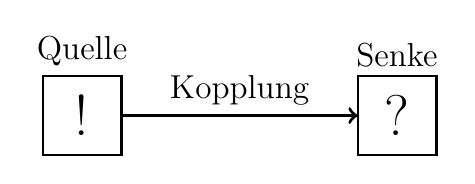
\begin{tikzpicture}
	\draw[thick] (-0.5,-0.5) rectangle (0.5,0.5); 
	\node at (0, 0) {\huge !};
	\node[above] at (0, 0.5) {\large Quelle};
	
	\draw[thick] (3.5,-0.5) rectangle (4.5,0.5);
	\node at (4, 0) {\huge ?};
	\node[above] at (4, 0.5) {\large Senke};
	
	\draw[->, very thick] (0.5, 0) -- node[above] {\large Kopplung} (3.5, 0);
\end{tikzpicture}
}\\
	%Autor: Simon Walker
%Version: 1.0
%Datum: 29.06.2020
%Lizenz: CC BY-NC-SA


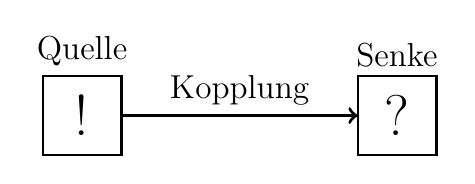
\begin{tikzpicture}
	\draw[thick] (-0.5,-0.5) rectangle (0.5,0.5); 
	\node at (0, 0) {\huge !};
	\node[above] at (0, 0.5) {\large Quelle};
	
	\draw[thick] (3.5,-0.5) rectangle (4.5,0.5);
	\node at (4, 0) {\huge ?};
	\node[above] at (4, 0.5) {\large Senke};
	
	\draw[->, very thick] (0.5, 0) -- node[above] {\large Kopplung} (3.5, 0);
\end{tikzpicture}
\\[5pt]
	Bei der Senke kann eigentlich nichts unternommen werden um Störungen zu vermeiden. Bei der Quelle kann man allfällige Störungen versuchen zu verhindern. Beispielsweise indem steile Flanken vermieden werden. Am meisten Einfluss haben wir allerdings auf die Kopplung. Wenn wir die Kopplung reduzieren wird die Störbeeinflussung ebenfalls reduziert.
\end{karte}

\begin{karte}{Welche Kopplungsarten von Störungen werden unterschieden?}
	Es gibt die kapazitive, die induktive, die galvanische und die Strahlen Kopplung.
\end{karte}
